\hypertarget{Tecnologie utilizzate}{%
\chapter{Tecnologie utilizzate}\label{tecnologie-utilizzate}}

\hypertarget{git-e-gitlab}{%
\section{Version control}\label{git-e-gitlab}}

Il progetto è stato portato avanti da un team di persone, quindi per coordinare il lavoro e i relativi cambiamenti al codice effettuati di volta in volta, si è scelto di utilizzare il software di \emph{version control} Git.

Tale software permette di tracciare i cambiamenti relativi ad un insieme di files, e viene utilizzato per coordinare il lavoro tra i programmatori nel team.

La gestione avviene all'interno di GitLab, ovvero  un provider di servizi che permette di gestire i progetti che utilizzano il software di controllo di versione Git. Permette di creare delle \emph{issues}, ovvero dei problemi che devono essere risolti, ed associare ad esse delle \emph{merge request.}

Una \emph{merge request} è un modo di controllare i cambiamenti effettuati nel codice presente in una \emph{feature branch} (\textit{branch} in cui si sta attualmente sviluppando una \textit{feature} o risolvendo un \textit{bug}) prima che questo venga unito al codice presente nella \emph{branch} principale.

Il \emph{branching} è un argomento fondamentale quando si parla di
\emph{version control} e di progetti che richiedono lo sviluppo contemporaneo di più persone all'interno di un \emph{team}.

Il \emph{branching}, in italiano ramificazione, consente agli sviluppatori di creare una copia del codice sorgente dell'applicazione, su cui lavorare per aggiungere una \emph{feature} o per risolvere un
\emph{bug}. I cambiamenti effettuati sulla \emph{feature branch} non impattano in nessun modo la \emph{branch} principale.

Una volta che il bug è stato risolto, o la feature implementata, e una volta che sono stati effettuati i dovuti test, il codice della
\emph{feature branch} può essere inserito nella \emph{branch} principale tramite l'operazione di \emph{merge}.

\hypertarget{concetti-fondamentali-di-unapplicazione-android}{%
\section{Componenti fondamentali in un'applicazione Android}\label{concetti-fondamentali-di-unapplicazione-android}}

In questa sezione vengono documentate le classi che sono fondamentali al fine di sviluppare un'applicazione Android.

\hypertarget{activity}{%
\subsection{Activity}\label{activity}}

Una \emph{activity} è una classe che permette di creare una finestra in cui è possibile specificare una determinata interfaccia grafica, il cui scopo è quello di permettere l’interazione tra il sistema e l’utente

Generalmente un'\emph{activity} è a schermo intero, ma questa può essere visualizzata anche come una finestra fluttuante oppure può essere inserita in un'altra finestra. \cite{activity}

Dal momento in cui l'\emph{activity} compare sullo schermo al momento in cui scompare, questa passa attraverso una serie di stati, in quella che viene chiamato \emph{activity lifecycle}, o ciclo di vita di una
\emph{activity}.

Un'activity presenta una serie di \emph{callbacks} che permettono alla activity stessa di capire che è avvenuto un cambio di stato all'interno dell'appicazione.

Queste funzioni, come ogni altra funzione in Java, possono essere
\emph{overwritten,} ovvero il loro comportamento può essere modificato, ed è quindi possibile specificare come l'activity debba comportarsi ad ogni cambio di stato. \cite{activity-lifecycle}

Una buona implementazione delle funzioni presenti nel ciclo di vita di una \emph{activity} permette all'applicazione di essere performante e robusta, ad esempio può evitare che l'app:

\begin{itemize}
    \item Vada in \emph{crash} se l'utente, ad esempio, mentre utilizza l'applicazione, riceve una telefonata e quindi l'applicazione deve essere eseguita in background;
    \item Consumi delle risorse di sistema preziose quando non ce n'è bisogno;
    \item Perda i progressi effettuati dall'utente quando questo esce e rientra in un secondo momento;
\end{itemize}
\begin{figure}[H]
\centering
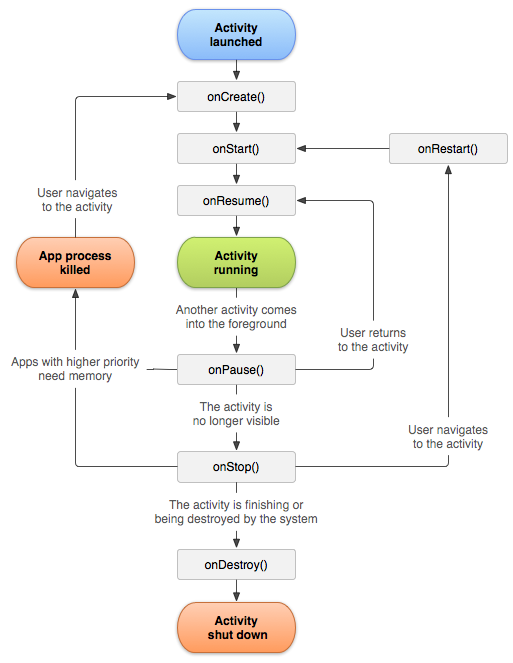
\includegraphics[width=12cm]{activity_lifecycle.png}
\caption{Ciclo di vita di una \emph{activity}}
\end{figure}


Una \emph{activity} implementa sei \emph{callbacks} fondamentali:

\begin{itemize}
    \item \texttt{onCreate}: viene chiamata quando il sistema crea l'activity, ed è all'interno di tale funzione che vengono effettuate le operazioni di inizializzazione che dovrebbero avvenire una sola volta durante l'intera vita dell'acivitiy;
    \item \texttt{onStart}: viene chiamata per rendere visibile l'activity all'utente, prima che essa venga eseguita in \emph{foreground} e diventi interattiva.
    \item \texttt{onResume}: viene chiamata ogni volta che l'attività deve essere eseguita in \emph{foreground}. L'attività rimane in questo stato finché non avviene un qualche evento che la porta in \emph{background}, come può essere una chiamata o l'apertura di un'altra applicazione.
    \item \texttt{onPause}: viene chiamata ogni volta che si presenta un evento che interrompe la normale esecuzione dell'activity. Questo non vuol dire che l'activity stia per essere distrutta, tantomeno che essa non sia più visibile dall'utente. Quando l'activity tornerà ad essere eseguita in \emph{foreground} verrà chiamata la funzione \texttt{onResume};
    \item \texttt{onStop}: viene chiamata quando l'activity non è più visibile dall'utente. L'activity in stato di \emph{stopped} è ancora presente in memoria. Da questo stato l'activity può tornare ad essere eseguita, e quindi verrà chiamata la funzione \texttt{onRestart}, oppure può essere distrutta, e quindi verrà chiamata la funzione \texttt{onDestroy};
    \item \texttt{onDestroy}: viene chiamata prima che l'activity venga distrutta, ed è lo stato finale del ciclo di vita dell'activity.
\end{itemize}
\hypertarget{fragment}{%
\subsection{Fragment}\label{fragment}}

Un Fragment rappresenta una porzione dell'interfaccia utente dell'applicazione. Esso definisce e gestisce il suo layout, ha un ciclo di vita proprio e può gestire i suoi eventi di input.

Un fragment non può tuttavia esistere da solo, ma deve essere inserito all'interno di un'activity o di un altro fragment.

I fragments rendono l'applicazione più modulare e riusabile, in quanto permettono di dividere la UI in più parti gestibili separatamente e riutilizzabili all'interno di diverse activities. \cite{fragments}

Dato che un fragment può esistere solo all'interno di una activity, il ciclo di vita di uno e dell'altra si innestano.

I cicli di vita del fragment quindi andranno di pari passo a quelli della activity in cui è inserito, e quindi il Fragment invocherà i metodi
\texttt{onCreate}, \texttt{onStart} e \texttt{onResume}. \cite{fragment-lifecycle} \cite{framents-lifecycle-2}

La classe fragment però possiede anche dei metodi propri, i più importanti sono:

\begin{itemize}
    \item \texttt{onAttach}: viene chiamato quando il Fragment viene aggiunto ad un \texttt{FragmentManager} ed è collegato all'activity ospite;
    \item \texttt{onCreateView}: viene chiamato per restituire la \texttt{View} in cui è presente il layout dell'interfaccia. Tra i parametri di input riceve un \texttt{LayoutInflater} la cui utilità è quella dell'eleborazione di un layout definito in un file .xml;
    \item \texttt{onActivityCreated}: in questo momento la creazione dell'activity è completa ed il fragment potrà interagire con essa;
    \item \texttt{onDestroyView}: indica la rimozione dell'interfaccia utente dal fragment, e prepara quest'ultimo allo scollegamento dall'activity;
    \item \texttt{onDetach}: viene chiamato quando il frammento viene rimosso dal \texttt{FragmentManager} e quindi scollegato dall'activity ospite.
\end{itemize}
\begin{figure}[H]
\centering
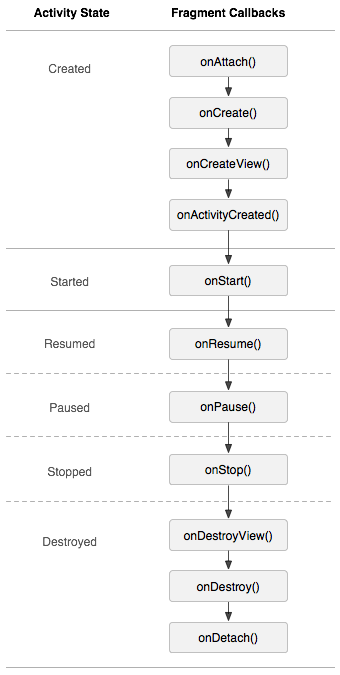
\includegraphics[width=8cm]{fragment_lifecycle.png}
\caption{Ciclo di vita di un \emph{fragment}}
\end{figure}

\hypertarget{intents}{%
\subsection{Intents}\label{intents}}

Un intent è un messaggio che viene usato da una componente dell'applicazione per richiedere un'azione da un'altra componente della stessa (o di un'altra) applicazione. \cite{intents}

Un intent può essere usato per:

\begin{itemize}
    \item Avviare un'activity;
    \item Avviare un \emph{service;}
    \item Inviare un messaggio in broadcast;
\end{itemize}
Esistono due tipi di \emph{intents}:

\begin{itemize}
    \item \textbf{Espliciti}: specificano quale componente verrà avviata per soddisfare l'intent. Un classico uso di un intent esplicito è per avviare un'activity a partire da un'altra activity;
    \item \textbf{Impliciti}: specificano solo un'azione generale, senza specificare la componente che andrà ad eseguire tale azione. Un esempio è quando si vuole effettuare un'azione tramite un'altra applicazione, e quindi si definisce l'azione, mostrando poi una finestra di dialogo in maniera tale che sia l'utente a scegliere con che applicazione eseguire tale azione.
\end{itemize}
\hypertarget{extras}{%
\subsubsection{Extras}\label{extras}}

Un intent porta con se delle coppie chiave-valore che possono essere inserite dalla componente che crea l'intent, e lette dalla componente che lo riceve.

\hypertarget{service}{%
\subsection{Service}\label{service}}

Un \emph{service} è una componente, non dotata di interfaccia grafica, all'interno di un'applicazione che permette di eseguire un operazione a lungo termine in \emph{background}. \cite{services}

Una volta eseguito, un \emph{service} può rimanere in esecuzione per un determinato lasso di tempo, anche in caso l'utente abbia cambiato applicazione.

Un \textit{service} può essere:
\begin{itemize}
    \item Foreground: esegue delle operazioni che possono essere notate dall'utente, ad esempio l'esecuzione di musica quando l'applicazione viene eseguita in background. Affinché il \textit{service} funzioni, l'applicazione deve mostrare un notifica durante tutta l'esecuzione del \textit{service};
    \item Background: esegue delle operazioni che non sono direttamente osservabili dall'utente, ad esempio la conversione da indirizzo sotto forma di stringa in coordinate.
\end{itemize}

\pagebreak


\hypertarget{gli-stati-dellutente}{%
\section{Gli stati dell'utente}\label{gli-stati-dellutente}}

L'applicazione implementa una macchina a stati finiti, il cui diagramma è mostrato di seguito.

\begin{figure}[H]
\centering
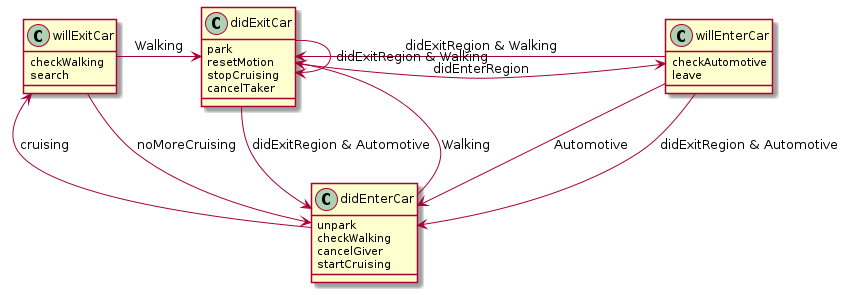
\includegraphics[width=12cm]{user_states.png}
\caption{Macchina a stati}
\end{figure}

Gli stati in cui può essere l'utente sono i seguenti:

\begin{itemize}
    \item \texttt{willExitCar}: l'utente ha parcheggiato e quindi sta per lasciare la macchina;
    \item \texttt{didExitCar}: l'utente ha parcheggiato dalla macchina ed è uscito da quest'ultima;
    \item \texttt{willEnterCar}: l'utente si sta avvicinando alla macchina a piedi e sta per entrare;
    \item \texttt{didEnterCar}: l'utente è entrato nella macchina parcheggiata e sta per uscire dal parcheggio.
\end{itemize}

\hypertarget{diagramma-uml-delle-classi}{%
\section{Diagramma UML delle classi}\label{diagramma-uml-delle-classi}}

Di seguito viene mostrato il diagramma UML delle delle classi, in cui vengono rappresentate le classi con cui il tirocinante ha interagito per l'implementazione delle funzionalità.

Le classi rappresentate da rettangoli a sfondo blu rappresentano le classi che sono state create durante il tirocinio, le altre rappresentano classi già esistenti nel progetto, che sono state inserite nel diagramma in quanto citate all'interno della relazione.

\begin{figure}[H]
\centering
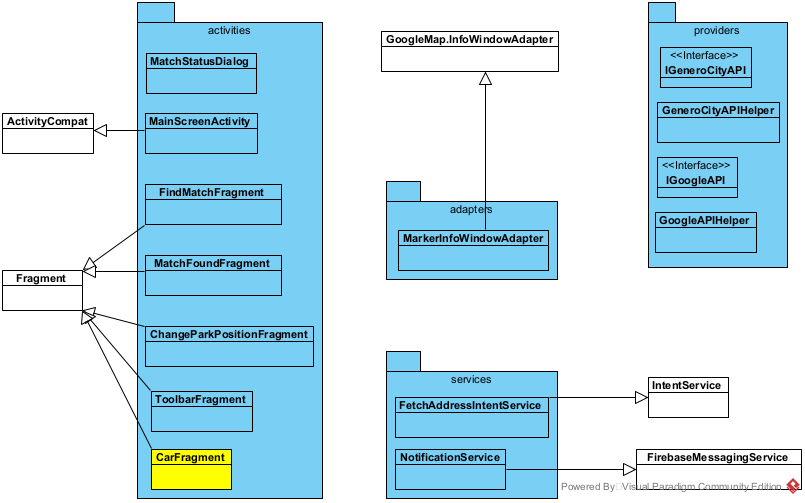
\includegraphics[width=12cm]{class_diagram.png}
\caption{Diagramma UML delle classi}
\end{figure}

\hypertarget{librerie-android-utilizzate}{%
\section{Librerie Android Utilizzate}\label{librerie-android-utilizzate}}

\hypertarget{retrofit}{%
\subsection{Retrofit}\label{retrofit}}

Retrofit è una libreria Java che permette di gestire in maniera semplice chiamate e risposte ad API REST.

La libreria Retrofit necessità l'implementazione di tre tipologie di classi:

\begin{itemize}
    \item Una classe per ogni oggetto che si vuole modellare, che verrà usata per la conversione da \texttt{json} ad oggetto java e viceversa;
    \item Un'interfaccia nella quale vengono definite le possibili API da chiamare;
    \item Una classe che implementa l'interfaccia definita nel punto precedente, ed in cui viene creato il Client Retrofit.
\end{itemize}
All'interno dell'interfaccia, ogni metodo rappresenta una possibile chiamata alle API. Vengono usate delle annotazioni del tipo
\texttt{@GET(”/me/”)} per definire l'endpoint della chiamata alle API ed il metodo HTTP. \cite{retrofit}

All'interno della classe definita nel terzo punto, viene costruito il Client nella seguente maniera

\begin{lstlisting} OkHttpClient client = httpClient.build(); 
Retrofit retrofit = new Retrofit.Builder()  
    .baseUrl(GCEnv.SERVER_URL)  
    .addConverterFactory(ScalarsConverterFactory.create())  
    .addConverterFactory(GsonConverterFactory.create(new GsonBuilder().excludeFieldsWithoutExposeAnnotation().create()))  
    .client(client) 
    .build();
return retrofit.create(IGeneroCityAPI.class);
\end{lstlisting}


\hypertarget{gson}{%
\subsection{Gson}\label{gson}}

\texttt{Gson} è una libreria Java (nel progetto integrata con Retrofit) che permette di convertire oggetti Java nella rappresentazione in oggetti \texttt{Json} e viceversa.

Tali oggetti Java modellano i vari elementi nel mondo reale trattati dal sistema. Gli oggetti rilevanti all'interno del lavoro svolto sono \texttt{Park} e \texttt{Match}. Visto che questi presentano un elevato numero di campi, di seguito verranno descritti quelli trattati maggiormente nel processo di sviluppo.

\hypertarget{park}{%
\subsubsection{Park}\label{park}}

Modella un parcheggio effettuato da un utente.

I campi più rilevanti sono:

\begin{itemize}
    \item \texttt{parktype}: indica il tipo di parcheggio, che può essere sconosciuto, a spina, parallelo o a pettine;
    \item \texttt{parkid}: intero che rappresenta il codice univoco del parcheggio;
    \item \texttt{parklat}: latitudine del parcheggio;
    \item \texttt{parklon}: longitudine del parcheggio;
    \item \texttt{starttime}: timestamp formattato come stringa che indica l'istante in cui l'utente ha parcheggiato;
    \item \texttt{endttime} timestamp formattato come stringa che indica l'istante in cui l'utente ha lasciato il parcheggio;
    \item \texttt{takerid}: codice univoco dell'utente che ha trovato il parcheggio tramite una ``ricerca posto''. Vale 0 se non esiste;
    \item \texttt{giverid}: codice univoco dell'utente che ha lasciato il posto tramite un ``lascia posto''. Vale 0 se non esiste.
\end{itemize}
\hypertarget{match}{%
\subsubsection{Match}\label{match}}

Modella un match, e presenta i seguenti campi:

\begin{itemize}
    \item \texttt{takerid}: codice univoco dell'utente Taker;
    \item \texttt{takercid}: codice univoco dell'auto con cui il Taker ha effettuato il match;
    \item \texttt{takerlat}: latitudine della posizione in cui il Taker intende trovare parcheggio;
    \item \texttt{takerlon}: longitudine della posizione in cui il Taker intende trovare parcheggio;
    \item \texttt{giverid}: codice univoco dell'utente giver
    \item \texttt{givercid}: codice univoco dell'auto con cui il Giver ha effettuato il match;
    \item \texttt{giverlat}: latitudine del parcheggio che il Giver intende lasciare;
    \item \texttt{giverlon}: longitudine del parcheggio che il Giver intende lasciare;
    \item \texttt{giverparkid}: codice univoco del parcheggio in cui è situata l'auto del giver;
    \item \texttt{parktype}: tipologia di parcheggio (si veda il campo omonimo in \texttt{park})
    \item \texttt{schedule}: timestamp che indica l'orario previsto in cui il Taker dovrebbe arrivare dal giver;
    \item \texttt{status}: indica lo stato del match nel momento corrente, il quale può assumere i seguenti valori:

 \begin{itemize}     \item  \texttt{waiting}: nel match è presente solamente il  Taker o il Giver in attesa che il sistema trovi un  utente con il ruolo opposto compatibile;     \item  \texttt{running}: il match è stato effettuato, e quindi sono  presenti sia Taker che Giver, ed è in corso di  esecuzione;     \item  \texttt{deleted}: il match, precedentemente in stato di  \texttt{waiting} è stato annullato dal Taker o dal Giver;     \item  \texttt{expired}: il match è scaduto perchè il Taker  non ha raggiunto la posizione del Giver entro 15 minuti;     \item  \texttt{success}: il match è stato completato con successo;     \item  \texttt{unsuccess-giver}: il match, precedentemente in  status di \texttt{running}, è stato annullato dal Giver;     \item  \texttt{unsuccess-taker}: il match, precedentemente in  status di \texttt{running}, è stato annullato dal Taker; \end{itemize}
    \item \texttt{updated}: timestamp formattato come stringa che indica l'istante in cui l'oggetto match ha ricevuto un aggiornamento di un qualche campo;
    \item \texttt{historyid}: codice univoco del match.
\end{itemize}
